\documentclass{beamer}
\usepackage[utf8]{inputenc}

\usetheme{Madrid}
\usecolortheme{default}
\usepackage{amsmath,amssymb,amsfonts,amsthm}
\usepackage{mathtools}
\usepackage{txfonts}
\usepackage{tkz-euclide}
\usepackage{listings}
\usepackage{adjustbox}
\usepackage{array}
\usepackage{tabularx}
\usepackage{gvv}
\usepackage{lmodern}
\usepackage{circuitikz}
\usepackage{tikz}
\usepackage{graphicx}
\setbeamertemplate{page number in head/foot}[totalframenumber]
\usepackage[T1]{fontenc}
\usepackage{tcolorbox}
\tcbuselibrary{minted,breakable,xparse,skins}

\definecolor{bg}{gray}{0.95}
\DeclareTCBListing{mintedbox}{O{}m!O{}}{%
  breakable=true,
  listing engine=minted,
  listing only,
  minted language=#2,
  minted style=default,
  minted options={%
    linenos,
    gobble=0,
    breaklines=true,
    breakafter=,,
    fontsize=\small,
    numbersep=8pt,
    #1},
  boxsep=0pt,
  left skip=0pt,
  right skip=0pt,
  left=25pt,
  right=0pt,
  top=3pt,
  bottom=3pt,
  arc=5pt,
  leftrule=0pt,
  rightrule=0pt,
  bottomrule=2pt,
  toprule=2pt,
  colback=bg,
  colframe=orange!70,
  enhanced,
  overlay={%
    \begin{tcbclipinterior}
    \fill[orange!20!white] (frame.south west) rectangle ([xshift=20pt]frame.north west);
    \end{tcbclipinterior}},
  #3,
}

% Code style
\lstset{
    language=C,
    basicstyle=\ttfamily\small,
    keywordstyle=\color{blue},
    stringstyle=\color{orange},
    commentstyle=\color{green!60!black},
    numbers=left,
    numberstyle=\tiny\color{gray},
    breaklines=true,
    showstringspaces=false,
}

% Title info
\title %optional
{5.2.21}
\date{October 4, 2025}
\author % (optional)
{EE25BTECH11018 - Darisy Sreetej}

\begin{document}

\frame{\titlepage}

\begin{frame}{Question}
Solve for the system of linear equations:
\begin{align*}
2x+ 3y= 13\\
4x + 5y= 23
\end{align*}
\end{frame}
\begin{frame}{Solution}
Let us solve the given question theoretically and then verify the solution computationally.\\
\\
According to the question,\\
The equation of lines given,
\begin{align}
    \myvec{2\\3}^\top\vec{x}=13 \\
    \myvec{4\\5}^\top\vec{x}=23
\end{align}
\begin{align}
    \therefore \myvec{2&&4\\3&&5}^\top\vec{x}=\myvec{13\\23}
\end{align}
\end{frame}
\begin{frame}{Solution}
Using augmented matrix,
\begin{align}
    \augvec{2}{1}{2&3&13\\4&5&23}
\end{align}
Upon doing row reduction,
\begin{align} 
     \augvec{2}{1}{2&3&13\\4&5&23}
     \xleftrightarrow{R_1 = \frac{1}{2}\times R_1}
     \augvec{2}{1}{1&\frac{3}{2}&\frac{13}{2}\\4&5&23}
\end{align}
\begin{align}
    \augvec{2}{1}{1&\frac{3}{2}&\frac{13}{2}\\4&5&23}
     \xleftrightarrow{R_2 = R_2 - 4 \times R_1}
    \augvec{2}{1}{1&\frac{3}{2}&\frac{13}{2}\\0&-1&-3}
\end{align}
\end{frame}
\begin{frame}{Solution}
\begin{align}
      \augvec{2}{1}{1&\frac{3}{2}&\frac{13}{2}\\4&5&23}
     \xleftrightarrow{R_2 = - R_2}
     \augvec{2}{1}{1&\frac{3}{2}&\frac{13}{2}\\0&1&3}
\end{align}
\begin{align}
      \augvec{2}{1}{1&\frac{3}{2}&\frac{13}{2}\\4&5&23}
     \xleftrightarrow{R_1 = R_1 - \frac{3}{2} \times R_1}
     \augvec{2}{1}{1&0&2\\0&1&3}
\end{align}
\begin{align}
    \implies \vec{x}=\myvec{2\\3}
\end{align}
\vspace*{0.25cm}
From the figure, it is clearly verified that the theoretical solution matches with the computational solution.
\end{frame}
\begin{frame}{Plot}
    \centering
    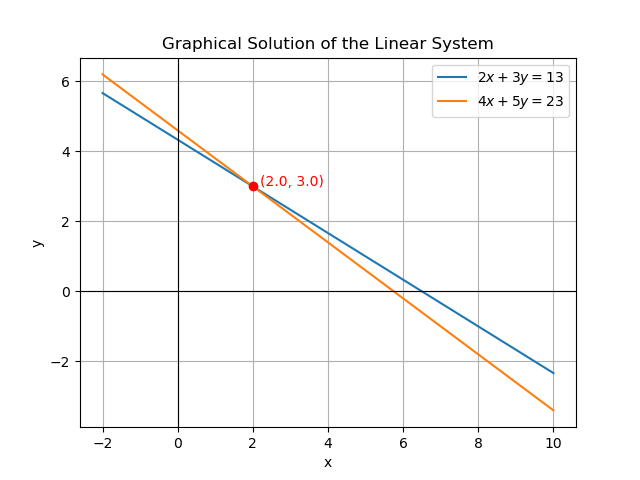
\includegraphics[width=3\columnwidth, height=0.8\textheight, keepaspectratio]{figs/fig.png}     
\end{frame}
\begin{frame}[fragile]
\frametitle{C code}
    \begin{lstlisting}[language=C]
#include <stdio.h>

void rref_solver(double aug[2][3], double solution[2]) {
    // Normalize first row (pivot = aug[0][0])
    double pivot = aug[0][0];
    for (int j = 0; j < 3; j++) {
        aug[0][j] /= pivot;
    }
    // Eliminate below pivot
    double factor = aug[1][0];
    for (int j = 0; j < 3; j++) {
        aug[1][j] -= factor * aug[0][j];
    }
\end{lstlisting}
\end{frame}
\begin{frame}[fragile]
    \frametitle{C Code }
    \begin{lstlisting}[language=C]
    //Normalize second row (pivot = aug[1][1])
    pivot = aug[1][1];
    for (int j = 0; j < 3; j++) {
        aug[1][j] /= pivot;
    }

    // Eliminate above pivot
    factor = aug[0][1];
    for (int j = 0; j < 3; j++) {
        aug[0][j] -= factor * aug[1][j];
    }

    //  Extract solution
    solution[0] = aug[0][2]; // x
    solution[1] = aug[1][2]; // y
}

     \end{lstlisting}
\end{frame}
\begin{frame}[fragile]
    \frametitle{Python + C Code }
    \begin{lstlisting}[language=Python]
import ctypes
import numpy as np
import matplotlib.pyplot as plt
import matplotlib as mp
mp.use("TkAgg")

# Load the shared C library (adjust filename if needed)
lib = ctypes.CDLL("./line_solver.so")

# Define argument and return types
lib.rref_solver.argtypes = [ctypes.c_double * 6, ctypes.c_double * 2]

# Augmented matrix for system:
# 2x + 3y = 13
# 4x + 5y = 23
aug = (ctypes.c_double * 6)(2, 3, 13,   4, 5, 23)  # Flattened 2x3
solution = (ctypes.c_double * 2)()
    \end{lstlisting}
\end{frame}

\begin{frame}[fragile]
    \frametitle{Python + C code}

    \begin{lstlisting}[language=Python]
# Call C function
lib.rref_solver(aug, solution)

# Convert result to numpy vector (ensure flat)
x_sol = np.array([solution[0], solution[1]], dtype=float).flatten()
print("Solution vector from C:", x_sol)

# Plot lines
x_vals = np.linspace(-2, 10, 400)
y1 = (13 - 2*x_vals) / 3
y2 = (23 - 4*x_vals) / 5

plt.plot(x_vals, y1, label=r"$2x+3y=13$")
plt.plot(x_vals, y2, label=r"$4x+5y=23$")

# Plot solution point
plt.scatter(x_sol[0], x_sol[1], color="red", zorder=5)
    \end{lstlisting}
\end{frame}

\begin{frame}[fragile]
    \frametitle{Python + C code}

    \begin{lstlisting}[language=Python]
plt.text(float(x_sol[0]) + 0.2, float(x_sol[1]),
         f"({x_sol[0]:.1f}, {x_sol[1]:.1f})", color="red")

plt.xlabel("x")
plt.ylabel("y")
plt.title("Graphical Solution of the Linear System")
plt.axhline(0, color="black", linewidth=0.8)
plt.axvline(0, color="black", linewidth=0.8)
plt.legend()
plt.grid(True)

plt.show()
\end{lstlisting}
\end{frame}
\begin{frame}[fragile]
    \frametitle{Python code}
    \begin{lstlisting}[language=Python]
import numpy as np
import matplotlib.pyplot as plt
import matplotlib as mp
mp.use("TkAgg")

# Coefficient matrix and RHS vector
A = np.array([[2, 3],
              [4, 5]], dtype=float)
b = np.array([13, 23], dtype=float)

# Solve system Ax = b
x = np.linalg.solve(A, b)
print("Solution vector for the system of equations:", x)

# Prepare x values for plotting
x_vals = np.linspace(-2, 10, 400)
    \end{lstlisting}
\end{frame}
\begin{frame}[fragile]
    \frametitle{Python code}

    \begin{lstlisting}[language=Python]
# Express y in terms of x for both equations
y1 = (13 - 2*x_vals) / 3      # from 2x + 3y = 13
y2 = (23 - 4*x_vals) / 5      # from 4x + 5y = 23

# Plot both lines
plt.plot(x_vals, y1, label=r"$2x + 3y = 13$")
plt.plot(x_vals, y2, label=r"$4x + 5y = 23$")

# Mark the solution point
plt.scatter(x[0], x[1], color="red", zorder=5)
plt.text(x[0] + 0.2, x[1], f"({x[0]:.1f}, {x[1]:.1f})", color="red")

# Formatting
plt.xlabel("x")
plt.ylabel("y")
plt.title("Graphical Solution of the Linear System")
plt.axhline(0, color='black', linewidth=0.8)
           \end{lstlisting}
\end{frame}
\begin{frame}[fragile]
    \frametitle{Python code}

    \begin{lstlisting}[language=Python]
plt.axvline(0, color='black', linewidth=0.8)
plt.legend()
plt.grid(True)

plt.show()
    \end{lstlisting}
\end{frame}
\end{document}
